% PAA Evaluation 2: Implementation & Initial Results. Same theme and palette as eval1_presentation.tex.
% Order follows the brief: refresher -> implementation -> initial results vs baseline -> analysis -> remaining plan.
% 12 slides in total (11 + 1 backup).
\documentclass[aspectratio=169,9pt]{beamer}
\usetheme[progressbar=frametitle,numbering=fraction]{metropolis}
\usepackage[T1]{fontenc}
\usepackage{lmodern}
\usepackage{booktabs}
\usepackage{array}
\usepackage{tikz}
\usetikzlibrary{arrows.meta,positioning,fit,calc}
\newcolumntype{L}[1]{>{\raggedright\arraybackslash}p{#1}}

% Template palette (as in Eval 1)
\definecolor{ink}{HTML}{111827}
\definecolor{body}{HTML}{374151}
\definecolor{accent}{HTML}{1D4ED8}
\definecolor{soft}{HTML}{EFF4FF}
\definecolor{panel}{HTML}{F9FAFB}
\definecolor{rule}{HTML}{D1D5DB}
\definecolor{muted}{HTML}{6B7280}
\definecolor{warm}{HTML}{C2410C}
\definecolor{warmsoft}{HTML}{FFF1E8}
\definecolor{bad}{HTML}{B91C1C}
\definecolor{good}{HTML}{15803D}
\definecolor{mlp}{HTML}{93C5FD}
\setbeamercolor{frametitle}{bg=ink,fg=white}
\setbeamercolor{progress bar}{fg=accent,bg=rule}
\setbeamercolor{normal text}{fg=body,bg=white}
\setbeamercolor{alerted text}{fg=warm}
\setbeamercolor{block title}{bg=soft,fg=ink}
\setbeamercolor{block body}{bg=panel}
\setbeamerfont{block title}{series=\bfseries}
\setbeamertemplate{frame numbering}{\insertframenumber/\insertmainframenumber}

\newcommand{\x}{$\times$}
\newcommand{\think}{\texttt{\textless/think\textgreater}}
\newcommand{\hd}[1]{{\color{accent}\bfseries #1}}
% A titled panel: \panel{width}{title}{body}
\newcommand{\panel}[3]{%
  \begin{tikzpicture}
    \node[draw=rule,fill=panel,rounded corners=3pt,inner sep=6pt,text width=#1,align=left] {%
      {\color{accent}\bfseries #2}\\[2pt]#3};
  \end{tikzpicture}}

\begin{document}

% ============================================================ 1  Title
\begin{frame}[plain]
  \vspace*{0.9cm}
  {\color{accent}\scriptsize\bfseries PROGRAMMING AI ACCELERATORS \,//\, EVALUATION 2: IMPLEMENTATION \& INITIAL RESULTS}\\[8pt]
  {\Huge\bfseries\color{ink} Joules per Thought}\\[6pt]
  {\Large\color{body} Where a reasoning LLM's decoding energy goes, component by component}\\[6pt]
  {\color{accent}\rule{\textwidth}{1pt}}\\[10pt]
  \begin{tabular}{@{}lll@{}}
    \textbf{Aaditya Bhatia} & \textbf{Virat Garg} & \textbf{Nidhish Jain} \\
    {\color{muted}2023114012} & {\color{muted}2023101081} & {\color{muted}2023101071}
  \end{tabular}\\[8pt]
  {\small Repo: \texttt{github.com/Nidhishj/Energy-Benchmarking-for-Reasoning-Models-PAA-Project}}
  \vfill
  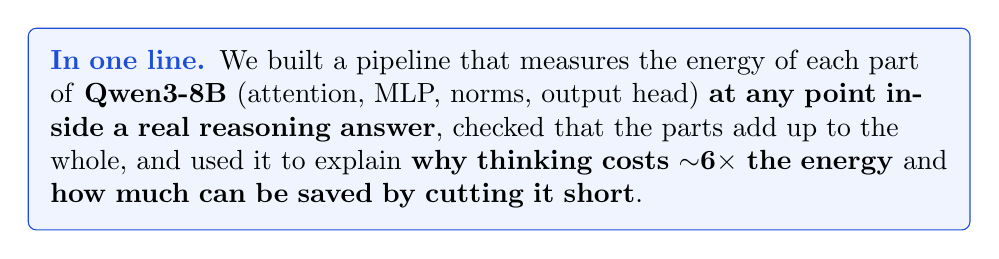
\begin{tikzpicture}
    \node[fill=soft,draw=accent,rounded corners=3pt,inner sep=8pt,text width=0.94\textwidth,align=left] {%
      {\color{accent}\bfseries In one line.} We built a pipeline that measures the energy of each part of
      \textbf{Qwen3-8B} (attention, MLP, norms, output head) \textbf{at any point inside a real reasoning answer}, checked
      that the parts add up to the whole, and used it to explain \textbf{why thinking costs $\sim$6\x\ the energy} and
      \textbf{how much can be saved by cutting it short}.};
  \end{tikzpicture}
  \vspace*{0.6cm}
\end{frame}

% ============================================================ 2  Refresher
\begin{frame}{Refresher: the problem, and what Evaluation 1 showed}
  \footnotesize
  \begin{columns}[T,onlytextwidth]
    \column{0.49\textwidth}
    \panel{0.93\textwidth}{The problem}{%
      \textbf{Reasoning models} (Qwen3 with ``thinking'' on) write a long hidden chain of thought before answering.
      Earlier studies measure only the \emph{whole model}: a reasoning answer costs several times a normal one, mainly
      because it is longer. \textbf{CLEAR} (Jain et al.) measures energy \emph{per component}, but only for short,
      fixed inputs.\\[2pt]
      \textbf{Our question}: as a reasoning answer grows, \textbf{which components} take its energy, does that differ for
      \textbf{wrong answers}, and can \textbf{cutting thinking short} lower the energy per correct answer?}\\[2pt]
    \panel{0.93\textwidth}{Why the hardware cares}{%
      Generating one token (a \textbf{decode step}, batch 1) reads all $\sim$16\,GB of weights for $\sim$1 FLOP per byte:
      \textbf{memory-bound}. Attention also reads the \textbf{KV cache} (stored keys/values of every earlier token,
      147\,KB each), which grows with every token.}
    \column{0.49\textwidth}
    \hd{Evaluation 1 baselines} {\scriptsize\color{muted}(RTX PRO 5000 Blackwell, Qwen3-8B BF16, 30 MATH-500 problems)}\\[2pt]
    \scriptsize
    \begin{tabular}{@{}L{0.17\textwidth}L{0.77\textwidth}@{}}
      \toprule
      \textbf{B1} & CLEAR's component method on BERT. Parts add up to only \textbf{74--88\%} of the whole (``\%Capture'').
        Our fix (sync before each reading, replay layers in their real order): \textbf{88--95\%}. \\
      \textbf{B2b} & Whole model, thinking on vs.\ off: \textbf{19.8 vs.\ 3.0\,kJ per answer} (6.5\x), 3{,}794 vs.\ 606 tokens,
        both 90\% accurate. Energy per token almost constant (5.16 vs.\ 4.96\,J). \\
      \textbf{B3} & Energy per token rises as the answer grows: \textbf{5.03 $\rightarrow$ 5.68\,J} from 512 to 8k tokens (+13\%). \\
      \bottomrule
    \end{tabular}
    \vspace{5pt}

    \hd{Plan we committed to} {\scriptsize\color{muted}(priority A $>$ B $>$ C)}
    \begin{itemize}\scriptsize\setlength{\itemsep}{1pt}
      \item \textbf{Exp A}: energy of each component at growing context; does attention take over?
      \item \textbf{Exp B}: per-component energy of \textbf{wrong vs.\ correct} answers.
      \item \textbf{Exp C}: force the end of thinking (\think) early; energy vs.\ accuracy.
      \item Plus: more problems (30 was too few to compare accuracy), a harder dataset, a higher token limit.
    \end{itemize}
  \end{columns}
\end{frame}

% ============================================================ 3  Implementation: what we built
\begin{frame}{Implementation (1/2): measuring components inside a real reasoning answer}
  \footnotesize
  \centering
  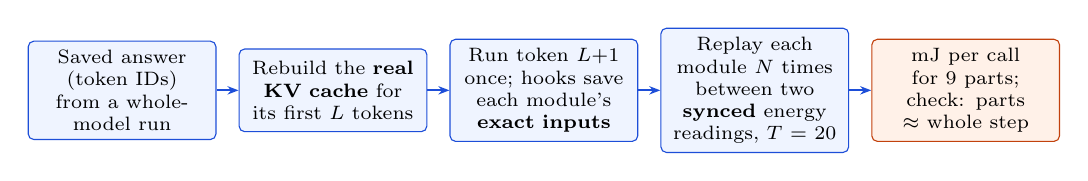
\begin{tikzpicture}[font=\scriptsize,node distance=0.28cm,
      box/.style={draw=accent,fill=soft,rounded corners=2pt,align=center,minimum height=1.05cm,text width=2.15cm},
      arr/.style={-{Stealth[length=4pt]},accent,thick}]
    \node[box] (t) {Saved answer (token IDs) from a whole-model run};
    \node[box,right=of t] (kv) {Rebuild the \textbf{real KV cache} for its first $L$ tokens};
    \node[box,right=of kv] (h) {Run token $L{+}1$ once; hooks save each module's \textbf{exact inputs}};
    \node[box,right=of h] (r) {Replay each module $N$ times between two \textbf{synced} energy readings, $T$ = 20};
    \node[box,right=of r,fill=warmsoft,draw=warm] (o) {mJ per call for 9 parts; check: parts $\approx$ whole step};
    \draw[arr] (t) -- (kv); \draw[arr] (kv) -- (h); \draw[arr] (h) -- (r); \draw[arr] (r) -- (o);
  \end{tikzpicture}\\[1pt]
  {\scriptsize\color{muted}$L$ = context length (tokens already in the KV cache). $N$ is set so one trial lasts $\sim$2\,s; energy from the GPU's own counter (NVML, mJ).\par}
  \vspace{4pt}
  \raggedright
  \begin{columns}[T,onlytextwidth]
    \column{0.33\textwidth}
    \panel{0.9\textwidth}{Exp A/B runner \texttt{expa/run\_decode\_components.py}}{%
      Parts of one decode step: input norm, \textbf{attention} (q/k/v/o, RoPE, KV read, SDPA), post norm, \textbf{MLP}, whole layer, embedding, final norm, \textbf{LM head}, and the \textbf{full step}.\\
      Attention sees exactly $L$ cached tokens on every replay (cache returned, not stored); the full step uses the real cache, cropped back after each call.
      Layer 18 measured, \x 36 for the model.}
    \column{0.33\textwidth}
    \panel{0.9\textwidth}{From one step to whole answers}{%
      \texttt{compare\_on\_off.py} prices \textbf{every saved answer token by token}: token $i$ costs the measured step at context
      prompt $+\,i$ (interpolated between measured $L$).
      Gives each answer's split into attention / MLP / norms / head, and a prediction to compare with its
      \textbf{measured} whole-model energy.}
    \column{0.33\textwidth}
    \panel{0.9\textwidth}{Exp C runners}{%
      \texttt{run\_expc.py}: replay a saved thinking trace, insert \think\ at 25/50/75\% of its length or at 512--4k tokens, sample the answer, measure.\\
      \texttt{run\_caps.py}: live caps ``think $\leq k$ tokens'' up to 16k on AIME.\\
      \texttt{stop\_rules.py}: offline test of rules that decide when to stop.}
  \end{columns}
  \vspace{4pt}
  {\scriptsize \hd{Also built}: 200-problem MATH-500 subset (40 per level) and \textbf{AIME 2024+2025} (60 problems, 32k-token limit);
  resumable runs (config hash, \texttt{--resume}); a GPU-busy guard; a \textbf{repro gate} that reruns 3 October problems on the baseline card
  before any new run; one-command run queues for a booked 6-hour slot.\par}
\end{frame}

% ============================================================ 4  Implementation: what ran, and is it valid
\begin{frame}{Implementation (2/2): what we ran, and the validity checks}
  \begin{columns}[T,onlytextwidth]
    \column{0.53\textwidth}
    \hd{Runs for Evaluation 2} {\scriptsize\color{muted}(Qwen3-8B, BF16, SDPA, batch 1)}\\[2pt]
    \scriptsize
    \begin{tabular}{@{}L{0.33\textwidth}L{0.40\textwidth}L{0.21\textwidth}@{}}
      \toprule
      Run & What & GPU \\
      \midrule
      Thinking on/off, MATH & 200 problems & Ada \\
      Thinking on/off, AIME & 60 problems \x 2 copies, $\leq$32k tok & Ada (2 cards) \\
      \textbf{Exp A}, wrong answer & AIME I-11, $L$ = 256--32k & Ada, PRO \\
      \textbf{Exp B}, correct answer & AIME I-8, $L$ = 256--16k & PRO \\
      \textbf{Exp B}, thinking off & AIME II-6 / I-10, $L \leq$ 8k & PRO / Ada \\
      Layer check & layers 0, 35 vs.\ 18 & PRO \\
      \textbf{Exp C}, MATH & 81 / 52 traces, 8 budgets & Ada / PRO \\
      Thinking caps, AIME & 2k/4k/8k/16k, 2 copies & Ada \\
      \bottomrule
    \end{tabular}\\[3pt]
    {\tiny\color{muted}RTX PRO 5000 Blackwell: 48\,GB, 1.34\,TB/s, 300\,W (the Eval 1 baseline card; one 6-h slot on 18 Nov).
    RTX 6000 Ada: 48\,GB, 0.96\,TB/s, 300\,W.\par}
    \column{0.44\textwidth}
    \hd{Validity checks} {\scriptsize\color{muted}(targets set in Eval 1)}\\[2pt]
    \scriptsize
    \begin{tabular}{@{}L{0.50\textwidth}L{0.42\textwidth}@{}}
      \toprule
      Check & Result \\
      \midrule
      Same card as Eval 1? Rerun 3 October problems & {\color{good}\textbf{PASS}}: within 4.6\% (limit 5\%) \\
      Parts add up to the whole step ($\geq$ 90\%) & \textbf{93.5--99.6\%} (PRO), 94--105\% (Ada) \\
      Trial-to-trial spread ($\leq$ 5\%) & \textbf{1--2\%} (PRO), 4--6\% (Ada) \\
      One layer represents all 36 & layers 0, 35 within \textbf{2.2\%} of 18 \\
      Two meters agree (Zeus vs.\ ours) & within 0.04\% \\
      Accuracy sample size & 200 + 60\x2 problems, 95\% ranges \\
      \bottomrule
    \end{tabular}
    \vspace{4pt}
    \begin{itemize}\scriptsize
      \item The October B1 fix carries over: on Qwen3-8B the parts add up \textbf{without} CUDA graphs (each module is large enough).
      \item Three dropped connections during the slot lost no data: every runner resumes.
    \end{itemize}
  \end{columns}
\end{frame}

% ============================================================ 5  Results 1: Exp A
\begin{frame}{Initial results (1/4) \,$\cdot$\, Exp A: attention takes over as the answer grows}
  \begin{columns}[T,onlytextwidth]
    \column{0.47\textwidth}
    \hd{Energy of one new token vs.\ context} {\scriptsize\color{muted}(full decode step)}\\[2pt]
    \centering
    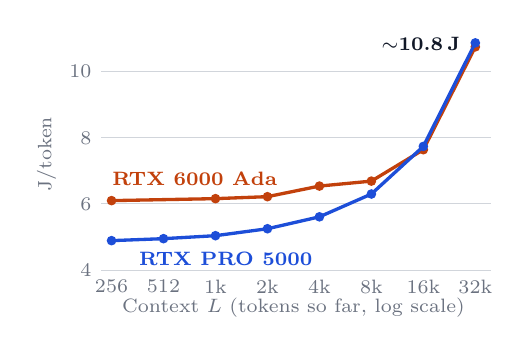
\begin{tikzpicture}[x=0.66cm,y=0.42cm,font=\scriptsize]
      \begin{scope}[shift={(0,-4)}]
        \foreach \v in {4,6,8,10} {
          \draw[rule] (-0.2,\v) -- (7.3,\v);
          \node[left,muted] at (-0.2,\v) {\v};
        }
        \foreach \i/\l in {0/256,1/512,2/1k,3/2k,4/4k,5/8k,6/16k,7/32k}
          \node[below,muted] at (\i,4) {\l};
        \node[muted] at (3.5,2.85) {Context $L$ (tokens so far, log scale)};
        \node[muted,rotate=90] at (-1.25,7.5) {J/token};
        \draw[warm,very thick] plot[mark=*,mark size=1.1pt] coordinates {(0,6.10) (2,6.16) (3,6.22) (4,6.54) (5,6.69) (6,7.64) (7,10.75)};
        \draw[accent,very thick] plot[mark=*,mark size=1.1pt] coordinates {(0,4.89) (1,4.95) (2,5.04) (3,5.25) (4,5.61) (5,6.30) (6,7.74) (7,10.87)};
        \node[warm,anchor=south,font=\scriptsize\bfseries] at (1.6,6.25) {RTX 6000 Ada};
        \node[accent,anchor=north,font=\scriptsize\bfseries] at (2.2,4.85) {RTX PRO 5000};
        \node[ink,anchor=east,font=\scriptsize\bfseries] at (6.9,10.85) {$\sim$10.8\,J};
      \end{scope}
    \end{tikzpicture}
    \raggedright
    \begin{itemize}\scriptsize
      \item Same answer (AIME I-11, thinking on), same contexts, two GPUs: \textbf{2.2\x\ the cost per token at 32k vs.\ 256}.
      \item PRO 5000 is 20\% cheaper at short context; at 32k the two cards are equal (slide 9).
    \end{itemize}
    \column{0.50\textwidth}
    \hd{Where that energy goes} {\scriptsize\color{muted}(RTX PRO 5000, J per token, whole model)}\\[2pt]
    \centering
    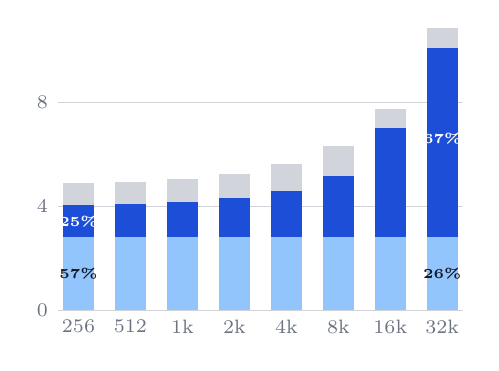
\begin{tikzpicture}[x=0.66cm,y=0.33cm,font=\scriptsize]
      \foreach \v in {0,4,8} {
        \draw[rule] (-0.4,\v) -- (7.4,\v);
        \node[left,muted] at (-0.4,\v) {\v};
      }
      \foreach \i/\a/\m/\r/\l in {0/1.23/2.80/0.86/256,1/1.29/2.80/0.86/512,2/1.35/2.82/0.87/1k,3/1.48/2.82/0.95/2k,
                                  4/1.76/2.82/1.03/4k,5/2.33/2.82/1.15/8k,6/4.21/2.80/0.73/16k,7/7.28/2.82/0.77/32k} {
        \fill[mlp] (\i-0.3,0) rectangle (\i+0.3,\m);
        \fill[accent] (\i-0.3,\m) rectangle (\i+0.3,\m+\a);
        \fill[rule] (\i-0.3,\m+\a) rectangle (\i+0.3,\m+\a+\r);
        \node[below,muted] at (\i,0) {\l};
      }
      \node[white,font=\tiny\bfseries] at (7,6.6) {67\%};
      \node[white,font=\tiny\bfseries] at (0,3.4) {25\%};
      \node[ink,font=\tiny\bfseries] at (0,1.4) {57\%};
      \node[ink,font=\tiny\bfseries] at (7,1.4) {26\%};
    \end{tikzpicture}\\[1pt]
    {\tiny\textcolor{accent}{\rule{7pt}{6pt}} attention (all 36 layers) \quad\textcolor{mlp}{\rule{7pt}{6pt}} MLP \quad\textcolor{rule}{\rule{7pt}{6pt}} norms, LM head, glue\par}
    \raggedright
    \begin{itemize}\scriptsize
      \item \textbf{Attention: 25\% $\rightarrow$ 67\%} of the step (1.2 $\rightarrow$ 7.3\,J). It is the only part that reads the KV cache, which reaches 4.8\,GB at 32k.
      \item \textbf{MLP is flat}: 78\,mJ per layer at every context (2.8\,J per token). LM head: 0.31\,J.
      \item Ada shows the same shape: attention 32\% $\rightarrow$ 63\%.
    \end{itemize}
  \end{columns}
\end{frame}

% ============================================================ 6  Results 2: against the baselines
\begin{frame}{Initial results (2/4) \,$\cdot$\, Comparison with the Evaluation 1 baselines}
  \begin{columns}[T,onlytextwidth]
    \column{0.50\textwidth}
    \hd{Do the parts rebuild the whole-model baseline?}\\
    {\scriptsize\color{muted}Every saved answer priced token by token with Exp A's costs, vs.\ the energy measured for that answer (B2b)\par}
    \vspace{3pt}
    \scriptsize\setlength{\tabcolsep}{3.5pt}
    \begin{tabular}{@{}llrrr@{}}
      \toprule
      Answers & GPU & Tokens & Predicted & \textbf{Pred./meas.} \\
      \midrule
      MATH, off & PRO & 457 & 3.0\,kJ & \textbf{99\%} \\
      MATH, on & PRO & 3{,}122 & 20.2\,kJ & \textbf{102\%} \\
      MATH, on, 8k cap & PRO & 8{,}192 & 46.0\,kJ & \textbf{105\%} \\
      \midrule
      MATH-200, off / on & Ada & 487 / 3{,}140 & 4.4 / 25.2 & 92 / 86\% \\
      AIME, off / on & Ada & 2{,}290 / 14{,}372 & 19.3 / 118.5 & 92 / 92\% \\
      \bottomrule
    \end{tabular}\\[1pt]
    {\tiny\color{muted}Tokens: median. PRO rows: the 90 + 90 Eval 1 baseline answers. Measured = the whole \texttt{generate()} call (prompt reading, sampling included).\par}
    \begin{itemize}\scriptsize
      \item \textbf{On the baseline card the components explain 99--105\% of B2b's measured energy.} On the Ada, 86--92\%: the rest is per-token work outside the model's forward pass (sampling, \texttt{generate()} bookkeeping), which is a larger share on that machine (slide 9).
    \end{itemize}
    \column{0.47\textwidth}
    \hd{Against each baseline}\\[2pt]
    \scriptsize
    \begin{tabular}{@{}L{0.17\textwidth}L{0.79\textwidth}@{}}
      \toprule
      \textbf{B1} CLEAR & CLEAR's way captured 74--88\% on BERT. Our method on Qwen3-8B decode: \textbf{93.5--99.6\%} at every context up to 32k. \\[2pt]
      \textbf{B2b} whole model & Repro of 3 October answers: within 4.6\%. Components rebuild per-answer energy (left). New: \textbf{200} MATH problems (off 86.0\%, on 85.5\%, 6.1\x\ energy) and \textbf{AIME} (left, next slides). \\[2pt]
      \textbf{B3} growth per token & Explained: the growth is \textbf{attention}. Live decoding rose +13\% from 512 to 8k; the replayed step rises +27\%. Whole answers still match (left), so the gap is at long context only: \textbf{open} (backup). \\
      \bottomrule
    \end{tabular}
    \vspace{6pt}

    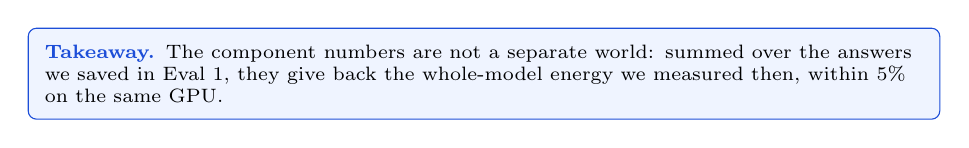
\begin{tikzpicture}
      \node[fill=soft,draw=accent,rounded corners=3pt,inner sep=6pt,text width=0.92\textwidth,align=left,font=\scriptsize] {%
        {\color{accent}\bfseries Takeaway.} The component numbers are not a separate world: summed over the answers we saved in Eval 1, they give back the
        whole-model energy we measured then, within 5\% on the same GPU.};
    \end{tikzpicture}
  \end{columns}
\end{frame}

% ============================================================ 7  Results 3: Exp B
\begin{frame}{Initial results (3/4) \,$\cdot$\, Exp B: wrong answers are not dearer per token, only longer}
  \begin{columns}[T,onlytextwidth]
    \column{0.46\textwidth}
    \hd{Same context, three kinds of answer} {\scriptsize\color{muted}(PRO 5000, J per token)}\\[2pt]
    \scriptsize
    \begin{tabular}{@{}rccc@{}}
      \toprule
      Context & Wrong (I-11) & Correct (I-8) & Thinking off (II-6) \\
      \midrule
      256 & 4.89 & 4.90 & 4.88 \\
      1k & 5.04 & 5.05 & 5.03 \\
      2k & 5.25 & 5.26 & 5.25 \\
      4k & 5.61 & 5.62 & 5.61 \\
      8k & 6.30 & 6.31 & 6.32 \\
      16k & 7.74 & 7.74 & -- \\
      \bottomrule
    \end{tabular}
    \begin{itemize}\scriptsize
      \item Within \textbf{0.4\%} at every context, and the component split matches too (attention 37--38\% at 8k).
      \item A token costs what its \textbf{position} costs, not what the answer turns out to be. (Ada, on vs.\ off: within 3\%.)
    \end{itemize}
    \column{0.51\textwidth}
    \hd{Whole answers: AIME 2024+2025} {\scriptsize\color{muted}(Ada, 120 answers per mode)}\\[2pt]
    \scriptsize
    \begin{tabular}{@{}lrrrr@{}}
      \toprule
      Answers & Median tok. & kJ / answer & Attention & MLP \\
      \midrule
      Thinking off & 2{,}290 & 19.3 & 35\% & 50\% \\
      Thinking on & 14{,}372 & 118.5 & 45\% & 44\% \\
      \quad on, correct (81) & 10{,}572 & 79.0 & 40\% & 47\% \\
      \quad \textbf{on, wrong (39)} & \textbf{28{,}614} & \textbf{200.5} & \textbf{48\%} & 42\% \\
      \bottomrule
    \end{tabular}\\[1pt]
    {\tiny\color{muted}kJ per answer predicted from components (92\% of measured for every row). Thinking on: 67.5\% correct vs.\ 25\% off, 6.2\x\ the energy.\par}
    \begin{itemize}\scriptsize
      \item A wrong thinking answer is \textbf{2.7\x\ longer} and costs \textbf{2.5\x} a correct one; more of it is attention.
      \item \textbf{The 33\% of thinking answers that are wrong use 55\% of thinking's energy.}
      \item On MATH-200 the effect is smaller (wrong: 36\% attention vs.\ 35\%) because answers stop at 8k tokens.
    \end{itemize}
  \end{columns}
\end{frame}

% ============================================================ 8  Results 4: Exp C
\begin{frame}{Initial results (4/4) \,$\cdot$\, Exp C: cutting thinking short}
  \begin{columns}[T,onlytextwidth]
    \column{0.47\textwidth}
    \hd{MATH: end thinking at a share of its own length}\\[2pt]
    \scriptsize
    \begin{tabular}{@{}lrrrr@{}}
      \toprule
      & \multicolumn{2}{c}{Ada (81 traces)} & \multicolumn{2}{c}{PRO 5000 (52)} \\
      Thinking kept & Acc. & Saved & Acc. & Saved \\
      \midrule
      100\% (full) & 100\% & -- & 100\% & -- \\
      75\% & 100\% & 22\% & 100\% & 22\% \\
      \textbf{50\%} & \textbf{100\%} & \textbf{43\%} & \textbf{100\%} & \textbf{43\%} \\
      25\% & 97.5\% & 64\% & 98.1\% & 65\% \\
      512 tokens & 95.1\% & 68\% & 96.2\% & 69\% \\
      none (off) & 95.1\% & 85\% & 98.1\% & 86\% \\
      \bottomrule
    \end{tabular}
    \begin{itemize}\scriptsize
      \item \textbf{Half of the thinking is enough on MATH}: 43\% less energy, no answer lost, same result on both GPUs.
      \item But MATH is easy for this model: thinking off is almost as accurate. The trade-off needs a harder set.
    \end{itemize}
    \column{0.50\textwidth}
    \hd{AIME: fixed caps ``think at most $k$ tokens''} {\scriptsize\color{muted}(120 answers)}\\[1pt]
    \centering
    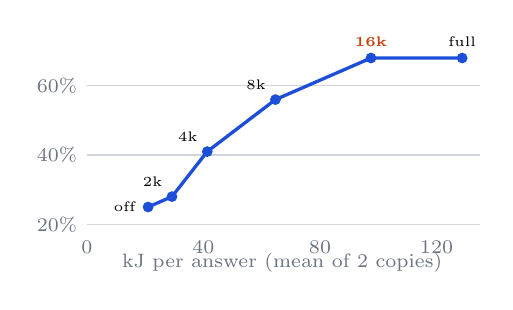
\begin{tikzpicture}[x=0.037cm,y=0.044cm,font=\scriptsize]
      \foreach \v in {20,40,60} {
        \draw[rule] (0,\v) -- (135,\v);
        \node[left,muted] at (0,\v) {\v\%};
      }
      \foreach \v in {0,40,80,120}
        \node[below,muted] at (\v,18) {\v};
      \node[muted] at (67,9) {kJ per answer (mean of 2 copies)};
      \draw[accent,very thick] plot[mark=*,mark size=1.3pt] coordinates {(21.0,25) (29.2,28) (41.3,41) (64.7,56) (97.5,68) (128.8,68)};
      \node[left,font=\tiny] at (20,25) {off};
      \node[above left,font=\tiny] at (29.2,28) {2k};
      \node[above left,font=\tiny] at (41.3,41) {4k};
      \node[above left,font=\tiny] at (64.7,56) {8k};
      \node[above,font=\tiny\bfseries,warm] at (97.5,68.5) {16k};
      \node[above,font=\tiny] at (128.8,68.5) {full};
    \end{tikzpicture}
    \raggedright
    \begin{itemize}\scriptsize
      \item On AIME every cut below 16k \textbf{costs accuracy}; a \textbf{16k cap keeps 68\%} and saves \textbf{22--26\%}.
      \item Stopping when two forced answers agree: 65\%, but the forced answers cost more than they save ($-$6 to $-$17\%).
        An oracle stop would save 18--28\% at 73\%: there is room for a better rule.
    \end{itemize}
  \end{columns}
\end{frame}

% ============================================================ 9  Analysis
\begin{frame}{Analysis: what profiling and the experiments taught us}
  \footnotesize
  \begin{columns}[T,onlytextwidth]
    \column{0.49\textwidth}
    \panel{0.93\textwidth}{1. On the PRO 5000, joules = 300\,W \x\ time}{%
      Step energy $\div$ step time = 298\,W at 256 tokens and 297\,W at 32k: the card runs \textbf{at its power limit}.
      So every millisecond saved per token is energy saved; 16.4 $\rightarrow$ 36.6\,ms per token is exactly the 2.2\x.}\\[1pt]
    \panel{0.93\textwidth}{2. Weights are a fixed cost, the KV cache grows}{%
      Every token reads $\sim$16.4\,GB of weights (MLP, projections: flat). The KV cache adds 147\,KB per earlier token:
      1.2\,GB at 8k, \textbf{4.8\,GB at 32k}. Attention's time per layer: 152 $\rightarrow$ 681\,$\mu$s.
      Hugging Face's cache also \textbf{copies the whole cache every step} (\texttt{torch.cat}), so attention moves
      $\sim$3\x\ the cache bytes; at 32k that is $\sim$0.75\,TB/s, about half the card's 1.34\,TB/s (our estimate).}
    \column{0.49\textwidth}
    \panel{0.93\textwidth}{3. The Ada server waits on its CPU at short context}{%
      Ada step time is \textbf{flat at 25.4\,ms from 256 to 8k} tokens while the KV cache grows 1.2\,GB, then rises.
      So at short context the GPU is not the bottleneck: it waits for the CPU to launch kernels (likely; not yet profiled),
      drawing 240\,W. Attention, many small kernels, is hit most: 401 vs.\ 152\,$\mu$s per layer at 256 tokens. Hence Ada is 25\% dearer at 256 tokens but equal at 32k, where both are GPU-bound.
      Part of Eval 1's Ada-vs-PRO gap is the host, not the GPU.}\\[1pt]
    \panel{0.93\textwidth}{4. Energy of an answer $\approx$ its length \x\ the average step cost}{%
      Cost per token depends only on position (slide 7), so answer energy = $\sum_i$ step$(L_i)$.
      Thinking costs $\sim$6\x\ because it is $\sim$6\x\ longer \textbf{and} its late tokens are dearer.
      Wrong answers are the longest, so they pay most for attention.}
  \end{columns}
  \vspace{3pt}
  {\scriptsize \hd{Smaller lessons}: one layer stands for all 36 (within 2.2\%); ``glue'' between modules is 0--11\% of a step;
  the Ada and PRO 5000 split energy the same way, so shares transfer across GPUs but joules do not.\par}
\end{frame}

% ============================================================ 10  Remaining plan
\begin{frame}{Remaining plan: comparisons, trade-offs, ablations}
  \footnotesize
  \begin{tabular}{@{}L{0.15\textwidth}L{0.55\textwidth}L{0.24\textwidth}@{}}
    \toprule
    & \textbf{What remains} & \textbf{Establishes} \\
    \midrule
    \hd{Comparisons} &
      \textbf{More traces per class}: Exp B has one correct, one wrong, one thinking-off answer. Add a second wrong (AIME II-8, 32k) and repeat on 3--5 each.\newline
      \textbf{Uncapped MATH-200}: rerun the 29 thinking and 18 non-thinking answers that hit the token limit (32k / 8k).\newline
      \textbf{Live vs.\ replayed step at 8--32k}: explain the B3 gap (+13\% vs.\ +27\%). &
      Exp B claim beyond one trace; accuracy and energy without truncation; whether the replay inflates long-context attention. \\[3pt]
    \hd{Trade-offs} &
      Energy vs.\ accuracy on AIME by \textbf{difficulty}: per problem group, the cheapest cap that keeps accuracy.\newline
      \textbf{A stopping rule that pays for itself}: short (e.g.\ 64-token) forced answers as probes, from 4k tokens on. &
      Energy per correct answer on a set where thinking matters. \\[3pt]
    \hd{Ablations} &
      \begin{tabular}{@{}L{0.17\textwidth}L{0.35\textwidth}@{}}
        KV cache & dynamic (copy every step) vs.\ \textbf{static} (pre-allocated) \\
        Attention kernel & SDPA vs.\ FlashAttention-2 vs.\ eager \\
        Measurement fixes & sync, in-order replay, CUDA graphs: one off at a time \\
        Host & same GPU step with a faster launch path (CUDA graphs) on the Ada \\
        Layer & 0 / 18 / 35 \;{\color{good}\bfseries done} (within 2.2\%) \\
      \end{tabular} &
      Is attention's growth inherent or a library cost? Which fix matters? Why the GPUs differ at short context. \\
    \bottomrule
  \end{tabular}
  \vspace{4pt}

  {\scriptsize \hd{Run budget}: the KV-cache and attention-kernel ablations reuse the Exp A runner ($\sim$1\,h per setting); the traces and caps
  reuse saved answers. One more PRO 5000 slot also finishes the last 2 of 54 Exp C traces.\par}
\end{frame}

% ============================================================ 11  Summary
\begin{frame}{Summary: built, learned, still to establish}
  \begin{block}{Key question}
    \textbf{Where does a reasoning model's decoding energy go}, as the answer grows and for wrong answers, and how much does \textbf{cutting thinking short} save?
  \end{block}
  \vspace{4pt}
  \footnotesize
  \begin{columns}[T,onlytextwidth]
    \column{0.32\textwidth}
    \panel{0.9\textwidth}{What we built}{%
      A component-energy pipeline for real decode steps at any point of a saved answer (parts add up: 93.5--99.6\%);
      per-answer pricing that reproduces the Eval 1 whole-model energy (99--105\%); thinking-budget runners;
      MATH-200 and AIME; resumable, repro-gated runs on two GPUs.}
    \column{0.32\textwidth}
    \panel{0.9\textwidth}{What we learned}{%
      \textbf{Attention grows from 25\% to 67\%} of a token's energy from 256 to 32k tokens; MLP is flat.
      \textbf{Per token, wrong = correct = thinking off}; wrong answers cost more only by being longer (55\% of AIME thinking energy).
      \textbf{Half the thinking} suffices on MATH ($-$43\%); on AIME a 16k cap saves 22--26\%.}
    \column{0.32\textwidth}
    \panel{0.9\textwidth}{Still to establish}{%
      Exp B over more traces; whether attention's growth survives a static KV cache and FlashAttention;
      the live-vs.-replay gap at long context; a stopping rule that beats a fixed cap on AIME; uncapped MATH-200.}
  \end{columns}
\end{frame}

% ============================================================ Backup (12th slide)
\appendix
\metroset{numbering=none}

\begin{frame}{Backup \,$\cdot$\, Caveats and numbers for questions}
  \begin{columns}[T,onlytextwidth]
    \column{0.49\textwidth}
    \hd{Caveats}
    \begin{itemize}\scriptsize
      \item \textbf{One answer per class} in Exp A/B so far (I-11 wrong, I-8 correct, II-6 off on PRO; I-10 off on Ada). The cost per token is set by the position, so more traces should agree; still to show.
      \item \textbf{Replay vs.\ live decoding at long context}: from 512 to 8k tokens the replayed step rises 27\%, live decoding (B3) 13\%. Up to 4k they agree within $\sim$5\%; whole answers within 5\%.
      \item Exp C thinking energy comes from a replay of the saved tokens, which reads $\sim$2\% low.
      \item MATH-200: 14.5\% of thinking answers stopped at 8{,}192 tokens, 9\% of non-thinking ones at 2{,}048; their energy is understated.
      \item The two cards differ in host machine and driver (560 vs.\ 595; both torch 2.8, transformers 4.57), so Ada-vs.-PRO joules mix GPU and host; shares do not depend on it.
      \item GPU-only energy from the card's counter; no wall meter. Idle power logged, not subtracted.
    \end{itemize}
    \column{0.48\textwidth}
    \hd{Exp A per-token numbers} {\scriptsize\color{muted}(J/token; ms/token)}\\[2pt]
    \scriptsize
    \begin{tabular}{@{}rrrrr@{}}
      \toprule
      Context & PRO 5000 & ms & Ada & ms \\
      \midrule
      256 & 4.89 & 16.4 & 6.10 & 25.5 \\
      1k & 5.04 & 17.0 & 6.16 & 25.4 \\
      4k & 5.61 & 18.9 & 6.54 & 25.3 \\
      8k & 6.30 & 21.2 & 6.69 & 25.4 \\
      16k & 7.74 & 26.0 & 7.64 & 29.0 \\
      32k & 10.87 & 36.6 & 10.75 & 40.8 \\
      \bottomrule
    \end{tabular}
    \vspace{4pt}

    \hd{Thinking on vs.\ off, whole model} {\scriptsize\color{muted}(Ada)}\\[2pt]
    \begin{tabular}{@{}lrrrr@{}}
      \toprule
      & \multicolumn{2}{c}{MATH-200} & \multicolumn{2}{c}{AIME (60 \x\ 2)} \\
      & off & on & off & on \\
      \midrule
      Accuracy & 86.0\% & 85.5\% & 25.0\% & 67.5\% \\
      kJ / answer & 4.8 & 29.1 & 20.9 & 128.7 \\
      kJ / correct & 5.5 & 34.0 & 83.7 & 190.7 \\
      \bottomrule
    \end{tabular}
  \end{columns}
\end{frame}

\end{document}
